\documentclass[12pt]{article}
 
\usepackage[margin=1in]{geometry} 
\usepackage{amsmath,amsthm,amssymb,outlines}
\usepackage{graphicx}
\usepackage{tikzsymbols}
\newenvironment{statement}[2][Statement]{\begin{trivlist}
\item[\hskip \labelsep {\bfseries #1}\hskip \labelsep {\bfseries #2.}]}{\end{trivlist}}

\begin{document}
 
\title{Homework 3} 
\author{}
\maketitle

\begin{statement}[Problem]{1}
  Show that composition of paths satisfies the following cancellation property: 
  If $f_0 \circ g_0 \cong f_1 \circ g_1$ and $g_0 \cong g_1$, then $f_0 \cong f_1$.
\end{statement}
\begin{proof}
  Let $g_0 \cong g_1$, so that there exists a homotopy $G_t$ 
  such that it is continuous, and $G_0 = g_0$ and $G_1 = g_1$. Similarly, there exists a continuous 
  $H_t$ such that $H_0 = f_0 \circ g_0$ and $H_1 = f_1 \circ g_1$. Then define $G^*_t(x)=G_t(1-x)$ so that $G^*_0(x)=G_0(1-x)=g_0(1-x)=\bar{g_0}(x)$ and $G^*_1(x)=G_1(1-x)=g_1(1-x)=\bar{g_1}(x)$. 
  Clearly, $G^*_t$ is continuous, so $\bar{g_0} \cong \bar{g_1}$.
  \par Note that $g_0 \circ \bar{g_0}$ and $g_1 \circ \bar{g_1}$ are the identity map, because they follow
  the path $g$ and then go back to the first endpoint when following $\bar{g}$. Then consider continuous $H_t \circ G^*_t$, where $H_0 \circ G^*_0 = f_0 \circ g_0 \circ \bar{g_0} = f_0$ and 
  $H_1 \circ G^*_1 = f_1 \circ g_1 \circ \bar{g_1} = f_1$. Thus $f_0 \cong f_1$. 
\end{proof}

\begin{statement}[Problem]{2}
  Show that the change-of-basepoint homomorphism $\beta_h$ depends only on the homotopy class of $h$.
\end{statement}
\begin{proof}
  Consider $\beta_h: \pi_1(X,x_1) \to \pi_1(X,x_0)$ and $\beta_{h'}: \pi_1(X,x_1) \to \pi_1(X,x_0)$, where the two paths, $h$ and $h'$, exist in the same homotopy class. 
  Both $h$ and $h'$ must have the same endpoints, $x_0$ and $x_1$, and there must exist a homotopy $H_t$, where $H_0 = h$ and $H_1 = h'$. 
  Thus for all $t \in [0,1]$, $H_t(x_1)=(x_0)$. Because $\beta_h$ maps $[f]$ to $[h \circ f \circ \bar{h}]$ and $\beta_{h'}$ maps 
  $[f]$ to $[h' \circ f \circ \bar{h'}]$, it is sufficient to show that $[h \circ f \circ \bar{h}] \cong [h' \circ f \circ \bar{h'}]$.
  \par First note that because $h$ and $h'$ are homotopic by $H_t$, there exists some $\bar{H_t}$ so that $\bar{h}$ and $\bar{h'}$ are homotopic as well.
  This is because we can define $\bar{H_t}(s)=H_t(1-s)$, so that it is continuous and $\bar{H_0}(s)=H_0(1-s)=h(1-s)=\bar{h}$, and $\bar{H_1}(s)=H_1(1-s)=h'(1-s)=\bar{h'}$.
  Then define $F_t=H_t(f)$, so that $F_0=H_0(f)=h \circ f$ and $F_1=H_1(f)=h' \circ f$, and $h \circ f \cong h' \circ f$. Similarly, we can define 
  $G_t = F_t \circ \bar{H_t}$, so that $G_0 = F_0 \circ \bar{H_0} = h \circ f \circ \bar{h}$, and $G_1 = F_1 \circ \bar{H_1} = h' \circ f \circ \bar{h'}$.
  Thus $h \circ f \circ \bar{h} \cong h' \circ f \circ \bar{h'}$, so that their homotopy classes are equal as well. 
\end{proof}

\begin{statement}[Problem]{3}
  For a path-connected space $X$, show that $\pi_1(X)$ is abelian iff all basepoint-change homomorphisms $\beta_h$ depend only
  on the endpoints of the path $h$.
\end{statement}
\begin{proof}
  $( \implies )$ Assume that $\pi_1(X)$ is abelian, so that for all $f,g \in \pi_1(X)$, $[f][g]=[f \circ g]=[g \circ f]=[g][f]$. 
  This is equivalent to saying that $f \circ g \cong g \circ f$. Let $h$ and $h'$ be paths with the same endpoints, and
  let $\bar{h}$ and $\bar{h'}$ be thier respective "reverses", like in problem 1. Then we know
  \begin{align*}
    f \circ g & \cong g \circ \bar{h'} \circ h' \circ f \\
          & \cong g \circ \bar{h'} \circ h \circ \bar{h} \circ h' \circ f \\
          & \cong ( g \circ \bar{h'} \circ h ) \circ ( \bar{h} \circ h' \circ f ) \\
          & \cong ( \bar{h} \circ h' \circ f ) \circ ( g \circ \bar{h'} \circ h ) \\
  \end{align*}
  Thus $h \circ f \circ g \circ \bar{h} \cong h' \circ f \circ g \circ \bar{h'}$, and so the basepoint-change homomorphisms
  only depend on the endpoints. Here is a visual of what is happening:
  \begin{center} 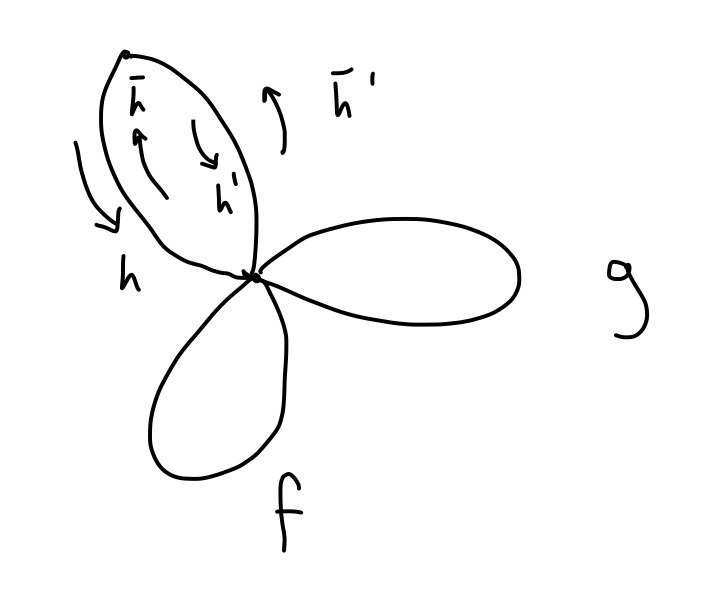
\includegraphics[scale=.3]{3.jpg} \end{center}
  \par $( \impliedby )$ Let $h$ be a constant loop and $\bar{h}$ it's reverse, and let $f,g \in \pi_1(X)$. Then note that $f \cong h \circ f \circ \bar{h}$, 
  but $h$ and $g$ have the same endpoints, because both are loops. Thus $f \cong h \circ f \circ \bar{h} \cong g \circ f \circ \bar{g}$. 
  Thus $\pi_1(X)$ is abelian. 
\end{proof}

\begin{statement}[Problem]{4}
  Show that for a space $X$, the following three conditions are equivalent:
  \begin{itemize}
    \item[(a)] Every map $S^1 \to X$ is homotopic to a constant map, with image a point. 
    \item[(b)] Every map $S^1 \to X$ extends to a map $D^2 \to X$. 
    \item[(c)] $\pi_1(X,x_0) = 0$ for all $x_0 \in X$. 
  \end{itemize}
\end{statement}
\begin{proof}
  First note that we already know $D^2$ is contractible.
  \begin{itemize}
    \item[$(a) \implies (b)$] Every map $S^1 \to X$ is homotopic to a constant map, call it $c:S^1 \to x_0$, where $x_0 \in X$. 
      We know $D^2$ is contractible, so that there exists a homotopy $H_t$ such that $H_0(x) = x$ and $H_1(x)=x_0$.
      Then we can extend $F_t$ to a map $G_t: D^2 \to X$, where $G_0(x)=f(x)$ and $G_1(x)=c$. 
    \item[$(b) \implies (c)$] By assumption, any loop on $S^1$ can be extended to a loop in $D^2$. Because $D^2$ is simply connected, 
      we know that any loop in $D^2$ can be contracted to any point $x_0 \in X$. Thus any loop is homotopic to a constant loop at $x_0$, 
      and so $\pi_1(X, x_0) = 0$. 
    \item[$(a) \implies (c)$] First note that the fundamental group being trivial tells us that all loops are homotopic to the constant loop,
      so all loops are contractible to a point. This is equivalent to saying all maps that are loops are homotopic to a constant function. 
      Thus it is sufficient to show that all maps $S^1 \to X$ are homotopic to loops. 
      \par Let $f$ be any map in $S^1 \to X$, with endpoints $f(0)=x_1$ and $f(1)=x_2$. If $x_1=x_2$, $f$ is a loop, we are done.
      If $x_1 \neq x_2$, we can simply define $g_1: [0,1] \to X$ such that $g_1(0) = x_0$ and $g_1(1)=x_1$, and 
      $g_2: [0,1] \to X$ such that $g_2(0) = x_2$ and $g_2(1)=x_0$. Thus $g_1 \circ f \circ g_2$ is a loop, and by assumption, homotopic to a constant function. 
      Because the homotopy between them must be continuous, $f$ must be homotopic to a constant function as well. 
      \par An image to describe what is happening here:
      \begin{center} 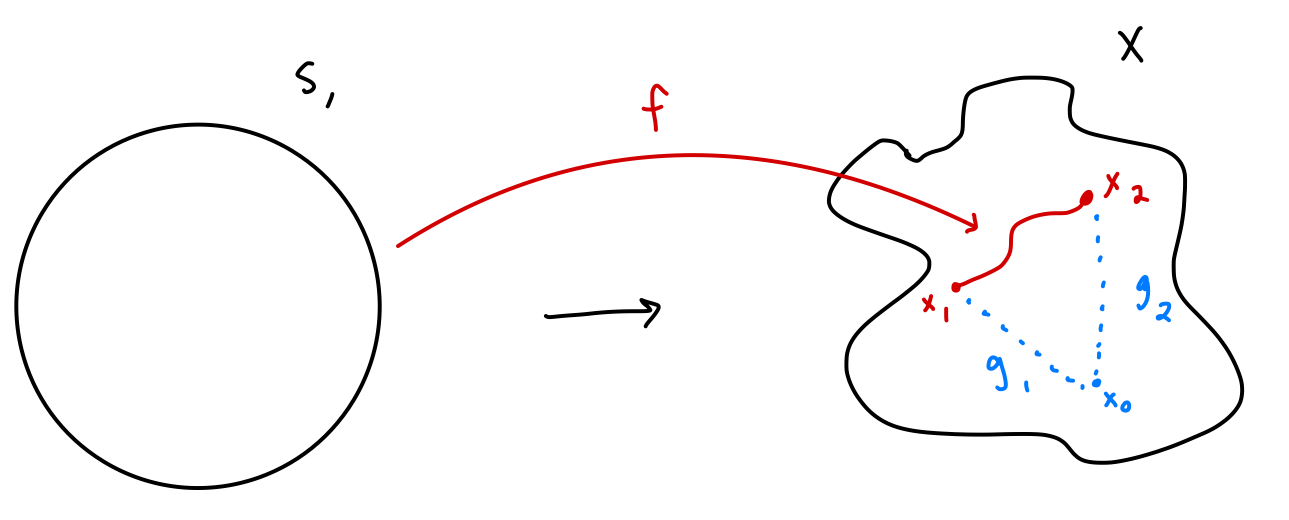
\includegraphics[scale=.3]{4.png} \end{center}
  \end{itemize}
\end{proof}

\begin{statement}[Problem]{5}
  Define $f:S^1 \times I \to S^1 \times I$ by $f(\theta, s)=(\theta + 2\pi s, s)$, so $f$ restricts to the identity on the
  two boundary circles of $S^1 \times I$. Show that $f$ is homotopic to the identity by a homotopy 
  $F_t$ that is stationary on one of the boundary circles, but not by any homotopy $F_t$ that is stationary on both boundary circles. 
\end{statement}
\begin{proof}
  
\end{proof}

\begin{statement}[Problem]{6}
  Show that there are no retractions $\mathcal{r}:X \to A$ in the following cases:
  \begin{itemize}
    \item[(a)] $X = \mathbb{R}^3$ with $A$ any subspace homeomorphic to $S^1$.
    \item[(b)] $X=S^1 \times D^2$ with $A$ its boundary torus $S^1 \times S^1$. 
    \item[(c)]$X = S^1 \times D^2$ with $A$ the circle shown in the figure.
    \item[(d)] $X = D^2 \vee D^2$ with $A$ its boundary $S^1 \vee S^1$.
    \item[(e)] $X$ a disk with two points on its boundary identified with $A$ and its boundary $S^1 \vee S^1$. 
    \item[(f)]$X$ the Mobius band and $A$ its boundary circle. 
  \end{itemize}
\end{statement}
\begin{proof}

\end{proof}

\begin{statement}[Problem]{7}
  Let $G$ be a topological group and $e \in G$ be the identity element. Show that $\pi_1(G,e)$ is abelian. 
\end{statement}
\begin{proof}

\end{proof}

\begin{statement}[Problem]{8}
  Let $H^1(X)=[X,S^1]$ denote the set of homotopy classes of continuous maps from $X$ to $S^1$. (There are no basepoints in this discussion)
  \begin{itemize}
    \item[(a)] Recall that $S^1$ is a topological group. Use the group structure on $S^1$ to make $H^1(X)$ into a group. Note that this group is abelian for any $X$. 
    \item[(b)] Compute $H^1(\text{{pt}})$.
    \item[(c)] Compute $H^1(S^1)$.
    \item[(d)] Show that $H^1$ is functional in the following sense: if $f: X \to Y$ is continuous then there is an induced homomorphism 
      $f^*H^1(Y) \to H^1(X)$. Moreover, if $g: Y \to Z$, then $(g \circ f)^* = f^* \circ g^*: H^1(Z) \to H^1(X)$.
    \item[(e)] Show that if $f ~ g$ then $f^* = g^*$. Conclude that if $X \cong Y$ then $H^1(X) \cong H^1(Y)$.
    \item[(f)] Use $H^1$ to prove that there is no retraction $D^2 \to S^1$, the key step in proving the Brouwer fixed point theorem.  
  \end{itemize}
\end{statement}
\begin{proof}

\end{proof}



\end{document}
